\section{Members of the Crew}


\begin{quotex}
the first and fundamental principle of esoterism (i.e. of the way of experience of the reality of the spirit) can be rendered by the formula:

Learn at first concentration without effort; transform work into play; make every yoke that you have accepted easy and every burden that you carry light!
\flright{\textsc{Valentin Tomberg}, \emph{Meditations on the Tarot}}
\end{quotex}


\begin{wrapfigure}{rt}{.3\textwidth}
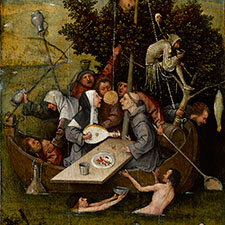
\includegraphics[width=.3\textwidth]{Hieronymus-Bosch_Ship-of-fools-225.jpg}
\end{wrapfigure}

Here we have a definition and a principle. Esoterism is the ``\emph{way of the experience of the reality of the spirit}''. Hence, there can be no ultimate ``esoteric interpretation'' of a text if by that is meant a verbal formulation. In spiritual works, there are four levels of interpretation:

\begin{itemize}


\item The historical or literal

\item The allegorical

\item The moral

\item The anagogical
\end{itemize}


They may each be true at their respective levels. Hence the idea that there is a ``truer'' esoteric interpretation that is opposed to the other levels is misguided. That is a common view, often used to sell books. On the contrary, the esoteric require an experience of the reality of the spirit, prior to any words and thoughts. And its proof is not a novel interpretation, but rather ``silence is the sign of real contact with the spiritual world''. To prepare for that, it is necessary to be:

\begin{itemize}


\item One in oneself, i.e., concentrated

\item One with the spiritual world, i.e., to have a zone of silence in the soul
\end{itemize}


This defies any sort of mechanical process. The exoteric believer prefers dogmas to believe, rules to follow, and commands to obey. At the exoteric level, this appears to be rational. Tomberg then makes this distinction:

\begin{quotex}
Evolution seen through the eyes of a passenger, i.e. seen as something which works by itself, is nevertheless not an illusion. That is. one can indeed find and prove the existence of a ``process of evolution'' or a ``progressive process'' which, on a phenomenological level, takes place by itself. But what effort, what sacrifices, what errors and what transgressions hide behind the phenomenological façade of the ``process of evolution'' and ``universal progress''---established and yet to be established. Here we have arrived at the heart of the ``exoterism --- esoterism'' problem.
\end{quotex}


In other words, there is flesh and blood behind this so-called process. To continue with the text:

\begin{quotex}
Exoterism lives in ``processes'', esoterism in tragedies and dramas. ... The ancient mysteries were tragedies and dramas--- it is here where their esoteric character lies. Exoterism corresponds to the mentality and psychology of a passenger, \textbf{esoterism to that of a member of the crew}.
\end{quotex}


On the esoteric path, you are called to be the actor in the tragedy and drama of your own life. The exoterists instead prefer to watch their lives unfold like a movie projected on a wall.

To return to the initial point about a ``secret'' interpretation, which is merely a disguised form of a new exoterism.

\begin{quotex}
Esoterism is therefore not a life and activity which seeks secrecy. It is based on the mentality and psychology of the crew, and its ``secrets'' are secrets only in so far as the mentality and psychology of the passengers is such as to refuse to participate in responsibility.
\end{quotex}


The passengers need to be guided. A fortiori, they need to be \emph{compelled}. On the one hand, they may desire proofs, or a case to be made. For example, proofs of God's existence, the soul, etc.

On the other hand, they look for a sign, or a miraculous event. Or, they expect God, the Holy Spirit, or and angel to select their life path. We have no objection to proofs or signs. Nevertheless, the esoterist chooses a different path. He makes his choice in total freedom and stands by it. Tomberg made this point in an earlier cycle of lectures published as \emph{Inner Development}. First of all, with a ``program'' to follow, his path is plagued with uncertainties:

\begin{quotex}
When we advance on the path of spiritual discipleship, we ourselves notice very little of this advance. Other people and higher beings notice it, but not we ourselves. We may be well aware of our mistakes and weaknesses, but it is not possible for us to know what we attain in the positive sense. Even the gods had to withdraw from their task and rest on the seventh day so that they could know that the world they had created was good. All the more so are human beings unable to say whether there is progress in their inner spiritual development. There is a sign, however, that does indicate this. It is the fact that one becomes inwardly ever more isolated. At first, one has many companions of the same disposition, awake to the same questions and concerns.
\end{quotex}


The esoterist then has no support from others, and especially not even visible support from above. This experience has been called the Dark Night, or facing the abyss, etc. Tomberg explains, presumably from his own experience:

\begin{quotex}
Then one discovers with dismay that the circle of people interested in these questions becomes ever narrower. Finally, one finds that there are only two or three others who are still awake in this domain---the others are asleep. At some point a person makes this discovery. Then there comes a moment at which one finds oneself alone between sleeping humanity and the dark, silent heavens. During the hour of the greatest decisions, heaven is silent---that is a law. \textbf{The spiritual beings do not want to impel a human being to any decision}. \textbf{As human beings, we must decide for ourselves, out of our freedom, everything that determines our destiny, our path}. And one can say that this situation---which was experienced to a tremendous degree by Christ Jesus---must be suffered through in some form or other by everyone on the path of spiritual discipleship.
\end{quotex}



\flrightit{Posted on 2018-11-10 by Cologero}

\begin{center}* * *\end{center}

\begin{footnotesize}
\begin{sffamily}

\texttt{Taivasvaeltaja on 2023-11-10 at 15:11 said:}

The adept is selfmade while the captain is visibly absent and other members of the crew don't reveal 
themselves.

\hfill

\end{sffamily}
\end{footnotesize}

